\begin{inhalt}
\renewcommand*\chapterpagestyle{scrheadings}
\chapter{Website}


\section{Signup}
\label{ref:Signup}
Für die Zuordnung der jeweiligen Benutzer ist es notwendig, dass sich die Nutzer einloggen können.  
Hierfür wurde eine Registrierkomponente erstellt, die den Registrier-Prozess ermöglicht.


\begin{figure}[!htb]
\centering
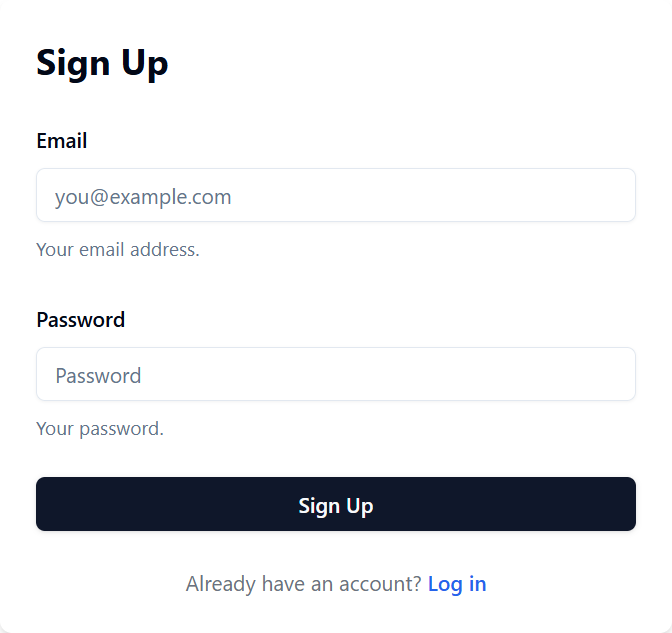
\includegraphics[width=0.5\textwidth]{files/Thomas/pics/Website/Signup/sign-up.png}
\caption[Bildbezeichnung für Abbildungsverzeichnis]{Registrierkomponente}
\label{fig:gehaeuse_internet_bild}
\end{figure}

Zur Validierung der Eingaben in den Feldern für \texttt{E-Mail} und \texttt{Passwort} wird die Bibliothek \textbf{Zod} verwendet. Dabei überprüft \textbf{Zod}, ob das E-Mail-Feld eine syntaktisch gültige E-Mail-Adresse enthält und ob das Passwortfeld einen String mit einer Mindestlänge von sechs Zeichen beinhaltet.


\begin{lstlisting}[style=mytsx]
const formSchema = z.object({
  email: z.string().email({
    message: "Please enter a valid email.",
  }),
  password: z.string().min(6, {
    message: "Password must be at least 6 characters.",
  }),
})
\end{lstlisting}
\index{Code Snippet 1@\hyperref[code:snippet1]{Snippet 1}}

\newpage

Für den Registrierungsvorgang wurde eine Funktion implementiert, die die eingegebene E-Mail-Adresse sowie das Passwort entgegennimmt und diese über eine Funktion des Supabase-Auth-Services im System registriert.


\begin{lstlisting}[style=mytsx]
export async function insert_user(email: string, password: string) {
  const supabase = await createClient();
  const { error } = await supabase.auth.signUp({
    email,
    password,
  });
  return error;
}
\end{lstlisting}

Nachdem der Nutzer erfolgreich registriert wurde, erfolgt eine Weiterleitung auf die Seite \texttt{/checkyouremails}, um ihn darüber zu informieren, dass er seine E-Mails überprüfen soll.

\begin{lstlisting}[style=mytsx]
      router.push("checkyouremails");
\end{lstlisting}

\subsection{Check Your Emails}

Auf dieser Seite wird überprüft, ob im Table \texttt{profiles} (siehe Referenz \ref{ref:profile-table-design}) das Feld \texttt{email\_confirmed\_at} gesetzt wurde und somit nicht mehr den Wert \texttt{null} enthält.  



\begin{figure}[H] 
  \centering
  \begin{subfigure}[b]{0.48\textwidth}
    \centering
    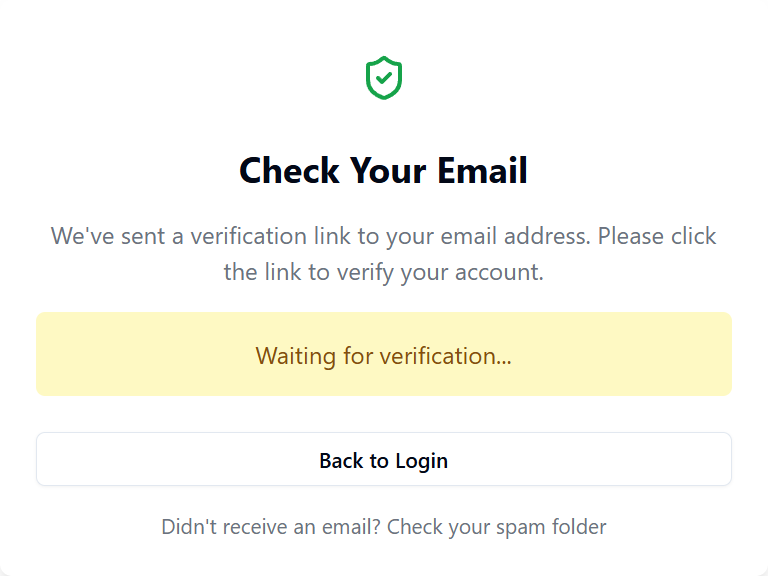
\includegraphics[width=1\textwidth]{files/Thomas/pics/Website/emailconfirmed/checkyouremails_waiting_verification.png}
    \caption{Email - Warte auf Verifikation}
    \label{fig:email_waiting_verification}
  \end{subfigure}
  \hfill
  \begin{subfigure}[b]{0.48\textwidth}
    \centering
    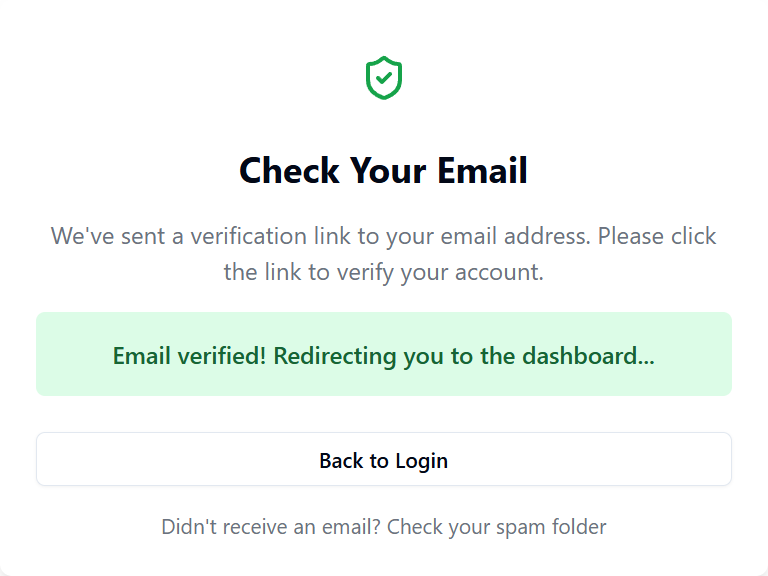
\includegraphics[width=1\textwidth]{files/Thomas/pics/Website/emailconfirmed/checkyouremails_verified.png}
    \caption{Email - Verifiziert}
    \label{fig:email_verified}
  \end{subfigure}
  \caption{Email Verifikation Status}
  \label{fig:email_verification_states}
\end{figure}


Dies geschieht über die Echtzeitfunktionalität von Supabase, welche es ermöglicht, Daten in Echtzeit zu aktualisieren und Änderungen in der Datenbank unmittelbar zu erkennen.

Sobald erkannt wird, dass die E-Mail-Adresse verifiziert wurde, erfolgt eine automatische Weiterleitung auf die \texttt{/login}-Seite.

\begin{lstlisting}[style=mytsx]
      router.push("/login");
\end{lstlisting}     


\section{Login}
\label{ref:Login}
Anschließend muss sich der Benutzer einloggen. Dieser Vorgang ist nahezu identisch mit dem Registrierungsprozess auf der \texttt{Sign-up}-Seite. 

\begin{figure}[!htb]
\centering
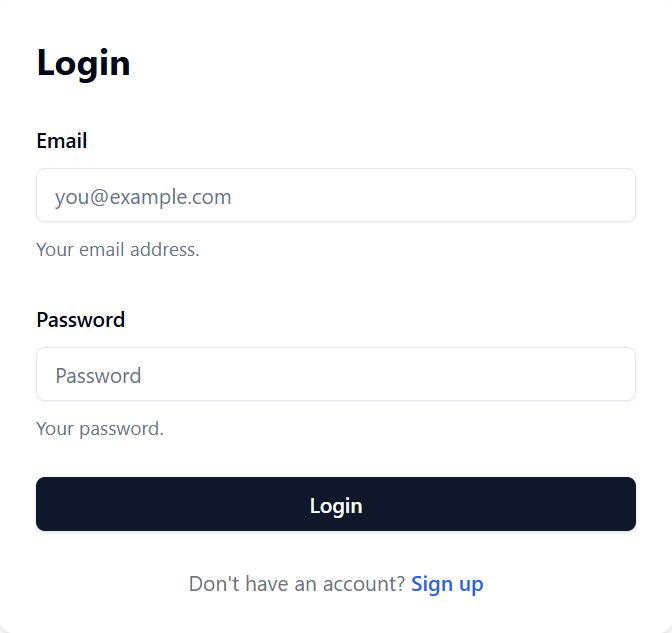
\includegraphics[width=0.5\textwidth]{files/Thomas/pics/Website/Login/login.png}
\caption[Bildbezeichnung für Abbildungsverzeichnis]{}
\label{fig:gehaeuse_internet_bild}
\end{figure}


Allerdings wird anstelle der \texttt{insert\_user}-Funktion zur Registrierung nun die \texttt{login\_user}-Funktion verwendet.
Da durch die E-Mail-Verifizierung keine automatische Benutzer-Session gestartet wird, muss der Benutzer sich manuell einloggen, um eine Session zu starten.

\begin{lstlisting}[style=mytsx]
export async function login_user(email: string, password: string) {
  const supabase = await createClient();
  const { error } = await supabase.auth.signInWithPassword({
    email,
    password,
  });
  return error;
}
\end{lstlisting}

\clearpage

\newpage

\section{Setup Profile}

Wenn ein Benutzer versucht, auf die \texttt{/setup-profile}-Seite zuzugreifen, und bereits angemeldet ist, wird überprüft, ob im Profil entweder der Benutzername, der Vorname oder der Nachname fehlt.  
Falls einer dieser Werte nicht gesetzt ist, wird der Benutzer automatisch durch die Middleware (siehe \ref{ref:middelware}) auf die entsprechende Seite weitergeleitet.

\vspace{0.25cm}

Die \texttt{/setup-profile}-Seite dient dazu, sicherzustellen, dass jeder Benutzer einen Benutzernamen, einen Vornamen und einen Nachnamen angegeben hat und diese Informationen vollständig vorliegen.

\begin{figure}[!htb]
\centering
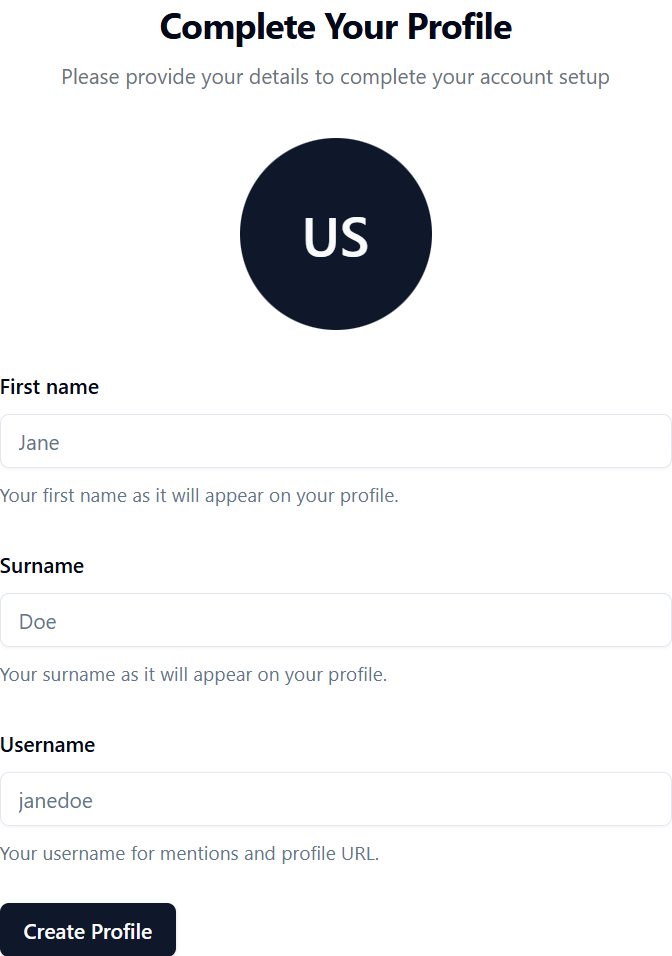
\includegraphics[width=0.55\textwidth]{files/Thomas/pics/Website/setup-profile/setup-profile.png}
\caption[Bildbezeichnung für Abbildungsverzeichnis]{}
\label{fig:gehaeuse_internet_bild}
\end{figure}

\clearpage

Diese Seite besteht ebenfalls aus einer Komponente, die ähnlich zur \texttt{Login}- und \texttt{Signup}-Komponente aufgebaut ist (siehe \ref{ref:Signup}, \ref{ref:Login}).

Der wesentliche Unterschied zwischen dem \texttt{Login}-Formular und der \texttt{Setup-Profile}-Seite besteht darin, dass auf der \texttt{Setup-Profile}-Seite zusätzlich ein Avatar hinzugefügt oder gelöscht werden kann.

\begin{lstlisting}[style=mytsx]
<AvatarUpload
    userName={form.getValues("first_name") || "User"}
    userId={userId || undefined}
    onImageChange={handleImageChange}
/>
\end{lstlisting}

\subsection{Funktionalitäten der AvatarUpload-Komponente}

Die \texttt{AvatarUpload}-Komponente stellt ein zentrales Element der Benutzerprofilseite (\texttt{/setup-profile}) dar. Sie ermöglicht eine intuitive Verwaltung von Profilbildern und gewährleistet eine konsistente visuelle Darstellung im gesamten System. Die Komponente implementiert vier Kernfunktionalitäten:

\vspace{1cm}

\textbf{Hochladen eines neuen Avatars mit Live-Vorschau}
\vspace{0.1cm}
Die Komponente ermöglicht das Hochladen von Profilbildern mit sofortiger Vorschau. Der Prozess umfasst:
\begin{itemize}
    \item Dateiauswahl aus dem lokalen Dateisystem
    \item Automatische Validierung (max. 5MB, nur Bildformate)
    \item Sofortige Vorschau ohne direkten Server-Upload
\end{itemize}

\begin{lstlisting}[style=mytsx, caption={Implementierung des Avatar-Uploads mit Validierung}, label={lst:avatar_upload}]
const handleFileSelect = async (event: React.ChangeEvent<HTMLInputElement>) => {
  const file = event.target.files?.[0];
  if (!file || !validateFile(file)) return;

  try {
    const fileExtension = file.type === "image/jpeg" ? "jpg" : "png";
    const standardizedFile = new File(
      [file], 
      `avatar.${fileExtension}`, 
      { type: file.type }
    );
    const previewUrl = URL.createObjectURL(file);

    setState(prev => ({
      ...prev,
      selectedFile: standardizedFile,
      previewUrl,
      avatarAction: "upload"
    }));
  } catch (error) {
    toast({
      title: "Fehler",
      description: "Datei konnte nicht verarbeitet werden."
    });
  }
};
\end{lstlisting}

\subsubsection{Entfernen bestehender Avatare}
Ein vorhandenes Profilbild kann über eine dedizierte Schaltfläche entfernt werden:
\begin{itemize}
    \item Visuelles Feedback durch \texttt{X}-Symbol
    \item Sofortige Aktualisierung der Anzeige
    \item Markierung zur Löschung beim nächsten Speichervorgang
\end{itemize}

\begin{lstlisting}[style=mytsx, caption={Implementierung der Avatar-Löschung}, label={lst:avatar_delete}]
const handleRemoveAvatar = async () => {
  try {
    setState(prev => ({
      ...prev,
      selectedFile: null,
      previewUrl: null,
      avatarAction: "delete"
    }));
    
    window.dispatchEvent(new CustomEvent("avatarChanged", {
      detail: { userId, action: "delete" }
    }));
  } catch (error) {
    toast({
      title: "Fehler",
      description: "Avatar konnte nicht entfernt werden."
    });
  }
};
\end{lstlisting}

\subsubsection{Intelligente Fallback-Darstellung}
Bei fehlendem Profilbild generiert die Komponente automatisch einen visuellen Platzhalter:
\begin{itemize}
    \item Extraktion der Benutzerinitialen aus dem Namen
    \item Konsistente Darstellung im UI-Design
    \item Automatische Anpassung an verschiedene Namensformate
\end{itemize}

\begin{lstlisting}[style=mytsx, caption={Generierung der Fallback-Initialen}, label={lst:avatar_initials}]
const getInitials = (name: string): string => {
  if (!name) return "??";
  const parts = name.split(" ");
  return parts.length === 1
    ? parts[0].substring(0, 2).toUpperCase()
    : (parts[0].charAt(0) + parts[parts.length - 1].charAt(0)).toUpperCase();
};
\end{lstlisting}

\subsubsection{Echtzeit-Synchronisation}
Die Komponente nutzt Supabase Realtime für die Live-Synchronisation:
\begin{itemize}
    \item Automatische Aktualisierung bei externen Änderungen
    \item Effiziente Subscription-Verwaltung
    \item Robuste Fehlerbehandlung
\end{itemize}

\begin{lstlisting}[style=mytsx, caption={Implementierung der Echtzeit-Synchronisation}, label={lst:avatar_subscription}]
useEffect(() => {
  if (!userId) return;
  
  let mounted = true;
  const setupSubscription = async () => {
    try {
      const channel = await subscribeToAvatarChanges(userId, () => {
        if (mounted) refreshAvatar();
      });
      if (mounted) channelRef.current = channel;
    } catch (error) {
      console.error("Subscription fehlgeschlagen:", error);
    }
  };

  setupSubscription();
  return () => {
    mounted = false;
    if (channelRef.current) unsubscribe(channelRef.current);
  };
}, [userId]);
\end{lstlisting}

Die \texttt{AvatarUpload}-Komponente vereint somit moderne Webtechnologien mit benutzerfreundlicher Funktionalität und robuster Fehlerbehandlung. Durch die Verwendung von TypeScript und React-Hooks wird eine wartbare und typsichere Implementierung gewährleistet.







\newpage

\section{Middleware}
\label{ref:middelware}

Die Datei \texttt{middleware} ist ein zentraler Bestandteil der Anwendung und wird bei jedem Seitenaufruf ausgeführt.  
Sie übernimmt wichtige Aufgaben im Bereich Sicherheit, Weiterleitung und Zustandskontrolle der Anwendung.  

%\begin{figure}[!htb]
%\centering
%\includegraphics[width=1\textwidth]{files/Thomas/pics/Website/middleware/middleware.png}
%\caption[Bildbezeichnung für Abbildungsverzeichnis]{}
%\label{fig:middleware}
%\end{figure}

Die Middleware wird automatisch bei jedem Aufruf einer Seite ausgeführt, sofern der aufgerufene Pfad nicht explizit ausgeschlossen wurde.  
Dadurch lassen sich serverseitige Logiken zentral abbilden, wie z.\,B. Authentifizierungsprüfungen, Weiterleitungen oder Cookie-Handling.

\subsection*{Wichtige Funktionen der Middleware}

\begin{enumerate}[label=\textbf{\arabic*.}]
  \item \textbf{Authentifizierung und Autorisierung}
  \begin{itemize}
    \item Überprüfung, ob ein Benutzer eingeloggt ist, mittels \texttt{supabase.auth.getUser()}
    \item Nicht eingeloggte Benutzer werden zur Login-Seite weitergeleitet
    \item Eingeloggte Benutzer, die sich auf Auth-Seiten befinden (z.\,B. \texttt{/login}, \texttt{/signup}), werden automatisch zum Dashboard umgeleitet
  \end{itemize}

  \item \textbf{Profilüberprüfung}
  \begin{itemize}
    \item Die Middleware prüft, ob das Benutzerprofil vollständig ist (Vorname, Nachname, Benutzername)
    \item Bei unvollständigem Profil erfolgt eine Weiterleitung zur \texttt{/setup-profile}-Seite
  \end{itemize}

  \item \textbf{Admin-Berechtigungen}
  \begin{itemize}
    \item Für Admin-Routen (\texttt{/admin/*}) wird geprüft, ob der Benutzer die Rolle \texttt{admin} besitzt
    \item Andernfalls erfolgt eine automatische Weiterleitung zum Dashboard
  \end{itemize}

  \item \textbf{Cookie-Management}
  \begin{itemize}
    \item Es werden Standard-Cookies wie \texttt{theme} und \texttt{activeSchool} gesetzt
    \item Die Authentifizierung erfolgt mithilfe des Supabase-Cookie-Managements
  \end{itemize}

\newpage

  \item \textbf{Routing-Logik}
  Die Routing-Logik prüft anhand des Authentifizierungsstatus, ob ein Benutzer weitergeleitet werden muss:


\begin{lstlisting}[style=mytsx]
  if (!user) {
    // If user is not logged in
    const isAuthRoute = path === '/login' || 
                        path === '/signup' || 
                        path === '/checkyouremails'
    
    if (!isAuthRoute) {
      // Redirect unauthenticated users to login page
      const redirectUrl = new URL('/login', request.url)
      return NextResponse.redirect(redirectUrl)
    }
  } else {
    // If user is logged in
    const isAuthRoute = path === '/login' || 
                        path === '/signup' || 
                        path === '/'
    
    if (isAuthRoute) {
      // Redirect authenticated users to dashboard
      const redirectUrl = new URL('/dashboard', request.url)
      return NextResponse.redirect(redirectUrl)
    }

  \end{lstlisting}

  \item \textbf{Matcher-Konfiguration}
  Die \texttt{matcher}-Konfiguration legt fest, auf welchen Routen die Middleware ausgeführt werden soll in diesen Falle auf fast alle:

\begin{lstlisting}[language=TypeScript]
matcher: [
  '/((?!_next/static|_next/image|favicon.ico|public/|api/|.
  *\\.(?:svg|png|jpg|jpeg|gif|webp|js|css)$).*)',
]


\end{lstlisting}



\clearpage

\newpage

\section{Seitenleiste}

Die Seitenleiste ist für die Navigation zwischen den verschiedenen Klassen, Abteilungen und Schulen verantwortlich.  

Der Aufbau der Seitenleiste besteht aus den folgenden Komponenten:

\begin{itemize}
    \item school-swticher
    \item nav-departments-classes-devices
    \item nav-user
\end{itemize}

%%% Bild einfügen von der Struktur

\begin{figure}[!htb]
\centering
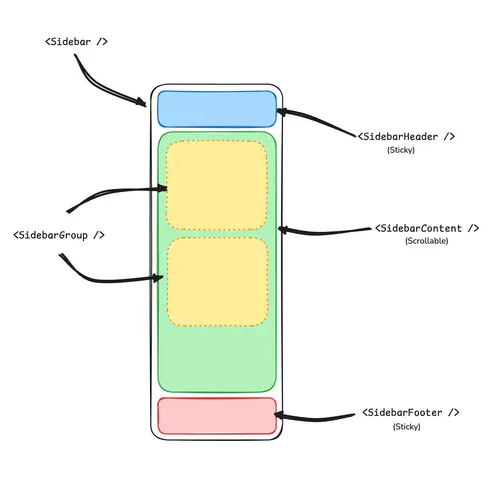
\includegraphics[width=1\textwidth]{files/Thomas/pics/Website/Sidebar/sidebar-aufbau.png}
\caption[Bildbezeichnung für Abbildungsverzeichnis]{}
\label{fig:gehaeuse_internet_bild}
\end{figure}

\newpage

\subsection{School-Switcher}

Die \texttt{school-switcher}-Komponente dient dazu, die aktuelle Schule auszuwählen bzw. zu wechseln.

\begin{figure}[!htb]
\centering

\includegraphics[width=1\textwidth]{files/Thomas/pics/Website/Sidebar/school-switcher/school-switcher.png}
\caption[School-Switcher Komponente geschlossen]{School-Switcher Komponente im geschlossenen Zustand}
\label{fig:school_switcher_closed}
\end{figure}

Administratoren können über einen Klick auf die Komponente ein Auswahlfenster öffnen, in dem sie zwischen den verfügbaren Schulen wählen können.  
Schüler, Lehrer und Direktoren besitzen hingegen keine Berechtigung, die Schule zu ändern.

\begin{figure}[!htb]
\centering
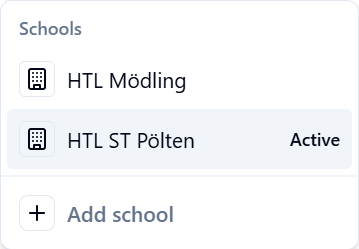
\includegraphics[width=0.75\textwidth]{files/Thomas/pics/Website/Sidebar/school-switcher/school-switcher-open.png}
\caption[School-Switcher geöffnet]{School-Switcher Komponente im geöffneten Zustand}
\label{fig:school_switcher_open}
\end{figure}

Die ausgewählte Schule wird anschließend in einem Cookie gespeichert, um beim nächsten Aufruf der Webseite automatisch wiederhergestellt zu werden.  
Im folgenden Codebeispiel wird das Cookie clientseitig unter dem Namen \texttt{activeSchool} gesetzt und speichert die \texttt{UUID} der Schul-ID.

Das Attribut \texttt{secure} sorgt dafür, dass das Cookie nur über HTTPS gesendet wird.  
Da dies jedoch nur in der Produktionsumgebung erforderlich ist, wird die Einstellung über \texttt{process.env.NODE\_ENV} gesteuert.  
Durch die Einstellung \texttt{sameSite = lax} wird das Cookie nur bei normaler Navigation und GET-Anfragen mitgesendet.  
Der Parameter \texttt{path} legt fest, dass das Cookie auf der gesamten Webseite verfügbar ist.

\begin{lstlisting}[language=TypeScript]
Cookies.set('activeSchool', school.id, {
    secure: process.env.NODE_ENV === 'production',
    sameSite: 'lax',
    path: '/',
});
\end{lstlisting}


%%% ADD School maby









\subsection{nav-departments-classes-devices}


\begin{figure}[!htb]
\centering
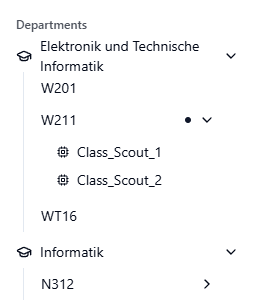
\includegraphics[width=0.5\textwidth]{files/Thomas/pics/Website/Sidebar/nav-departments-classes-devices/nav-screen.png}
\caption[Bildbezeichnung für Abbildungsverzeichnis]{}
\label{fig:gehaeuse_internet_bild}
\end{figure}



Die Aufgabe der nav-departments-classes-devices Komponente ist das Man zwischen den Abteilungen Klassen und Sensoren umher Navigiren kann. Damit erkannt wird in welcher Schule man sich Befindet wurde eine Speziele URL Addresse entworden:

\begin{lstlisting}[language=TypeScript]

domainname/uuid-der-schule/dashboard?department=uuid-in dem-Department-man-gerae-ist&class=uuid-in-welcher-Klasse-man-sich-gerade befindet&device=device-uuid

Beispiel

domainname/0d3e37cf-8350-46f2-823b-26dd90c01266/dashboard?department=e1ed2bd8-4c9c-40f8-bec7-4edcebe59fc1&class=eb4355fd-1e98-4961-be62-36fa9fc5cec0&device=a52eb8dc-5df5-475a-8a9f-f5f5a24ac2d3
\end{lstlisting}


%%% gehört vlt noch was hin 

\subsection{nav-user}

Die nav-user Komponente ist im SidebarFooter(Am Boden der Seitenleiste). Sie ist verantwortlich dafür das sie vom Benutzer den Benutzernamen die E-Mail Addresse den Avatar anzeigt

\begin{figure}[!htb]
\centering

\includegraphics[width=0.5\textwidth]{files/Thomas/pics/Website/Sidebar/nav-user/user-component.png}
\caption[Bildbezeichnung für Abbildungsverzeichnis]{}
\label{fig:gehaeuse_internet_bild}
\end{figure}

\clearpage

Außerdem ist es auch noch da um Auf den Profil Editor des Bentuzers zu kommen. Wenn man ein Admin ist kann man auch auf die Administrator Seiten der Website kommen und es gibt noch eine Settings Seite und einen Logout Knopf um sich abzumelden. 

\begin{figure}[!htb]
\centering
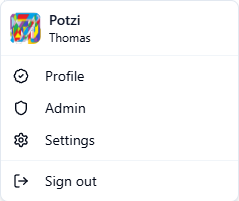
\includegraphics[width=0.5\textwidth]{files/Thomas/pics/Website/Sidebar/nav-user/user-component-open.png}
\caption[Bildbezeichnung für Abbildungsverzeichnis]{}
\label{fig:gehaeuse_internet_bild}
\end{figure}



Beim Abmelden von der Seite wird als erstes  gewarted bis die signOut funktion ein success zurück bekommt danach wird der user auf die Lgin seite weitergeleitet. 

\begin{lstlisting}[language=TypeScript]
  const handleSignOut = async () => {
    const { success, error } = await signOut();
    if (success) {
      router.push("/login");
    } else {
      console.error("Error signing out:", error);
    }
  };
\end{lstlisting}


\newpage

\section{Settings Seite}

\begin{figure}[!htb]
\centering
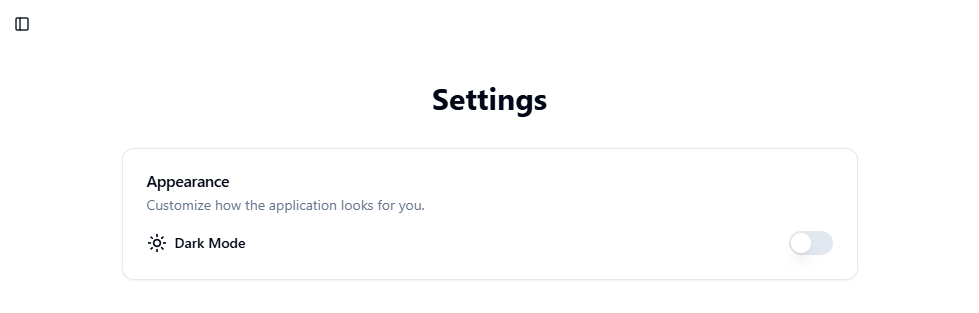
\includegraphics[width=1\textwidth]{files/Thomas/pics/Website/Settings/settings-screen.png}
\caption[Bildbezeichnung für Abbildungsverzeichnis]{}
\label{fig:gehaeuse_internet_bild}
\end{figure}


Die Settings(Einstellungs Seite hat nur eine Aufgabe und zward den Theme zu wechseln dieser wird dann wieder in den Cookies gespeichet mit den Namen theme um bei einen Refresh nicht den Theme zu verlieren.

\vspace{2cm}

In diesn Code wird ein Schalter eingesetzt um in den Dunklen Modus oder den Hellen Modus zu wechseln. Dieser Switch hat die id dark-mode und eine Variable die den Wert des Schalters annimt am Schluss wird jedes mal wenn der Schalter geschalten wird wird die Funktion "toggelTheme" aufgerufen um die Cookies und den Theme der Seite zu verändern.


\begin{lstlisting}[language=TypeScript]
<Switch
    id="dark-mode"
    checked={isDarkMode}
    onCheckedChange={toggleTheme}
  />
\end{lstlisting}

\newpage

\section{Profile Seite}

Die Profile Seite ist eigetnlich die Profile-Setup Seite um den Benutzer die Möglichkeit zu geben das Profil Bild den Vorname Nachnmaen und Bentuzernamen zu aktualisieren.


\begin{figure}[!htb]
\centering
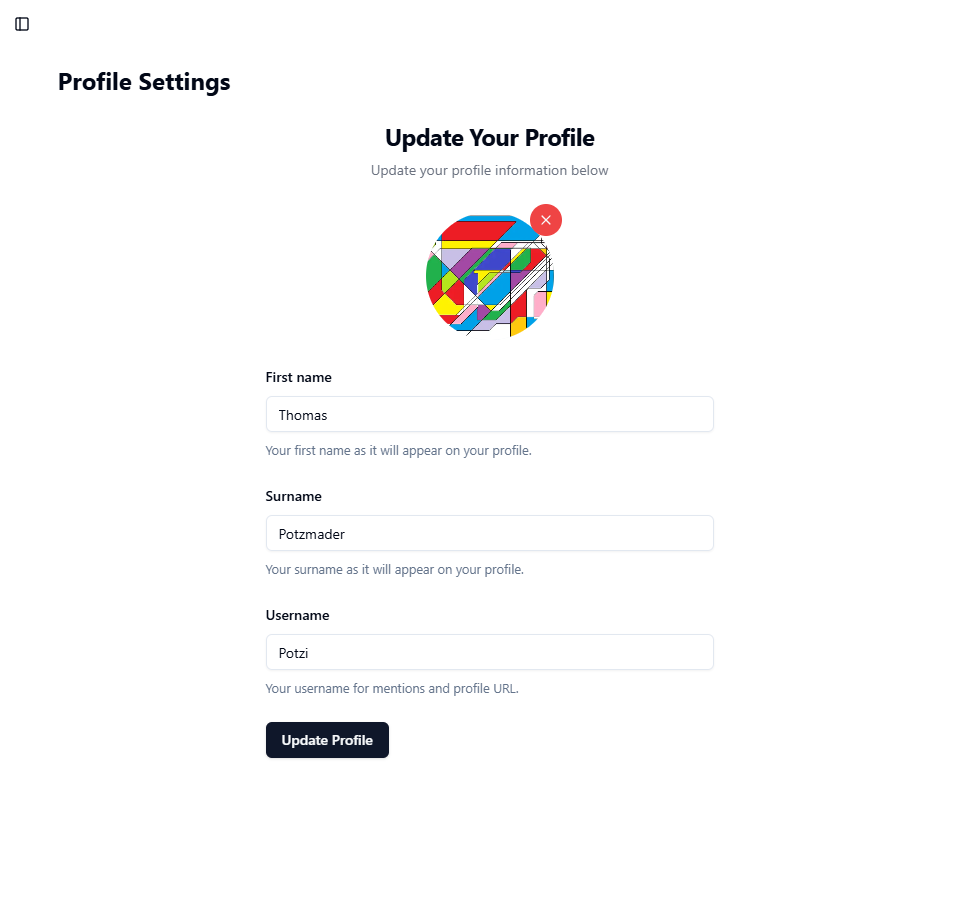
\includegraphics[width=1\textwidth]{files/Thomas/pics/Website/Profile/profile-screen.png}
\caption[Bildbezeichnung für Abbildungsverzeichnis]{}
\label{fig:gehaeuse_internet_bild}
\end{figure}

\newpage

\section{Admin Dashboard}

Das Admin Dashboard ist dafür da um alle User, Geräte, Klassen, Abteilungen und Schulen zu Erstellen oder zu Löschen. 

\begin{figure}[!htb]
\centering
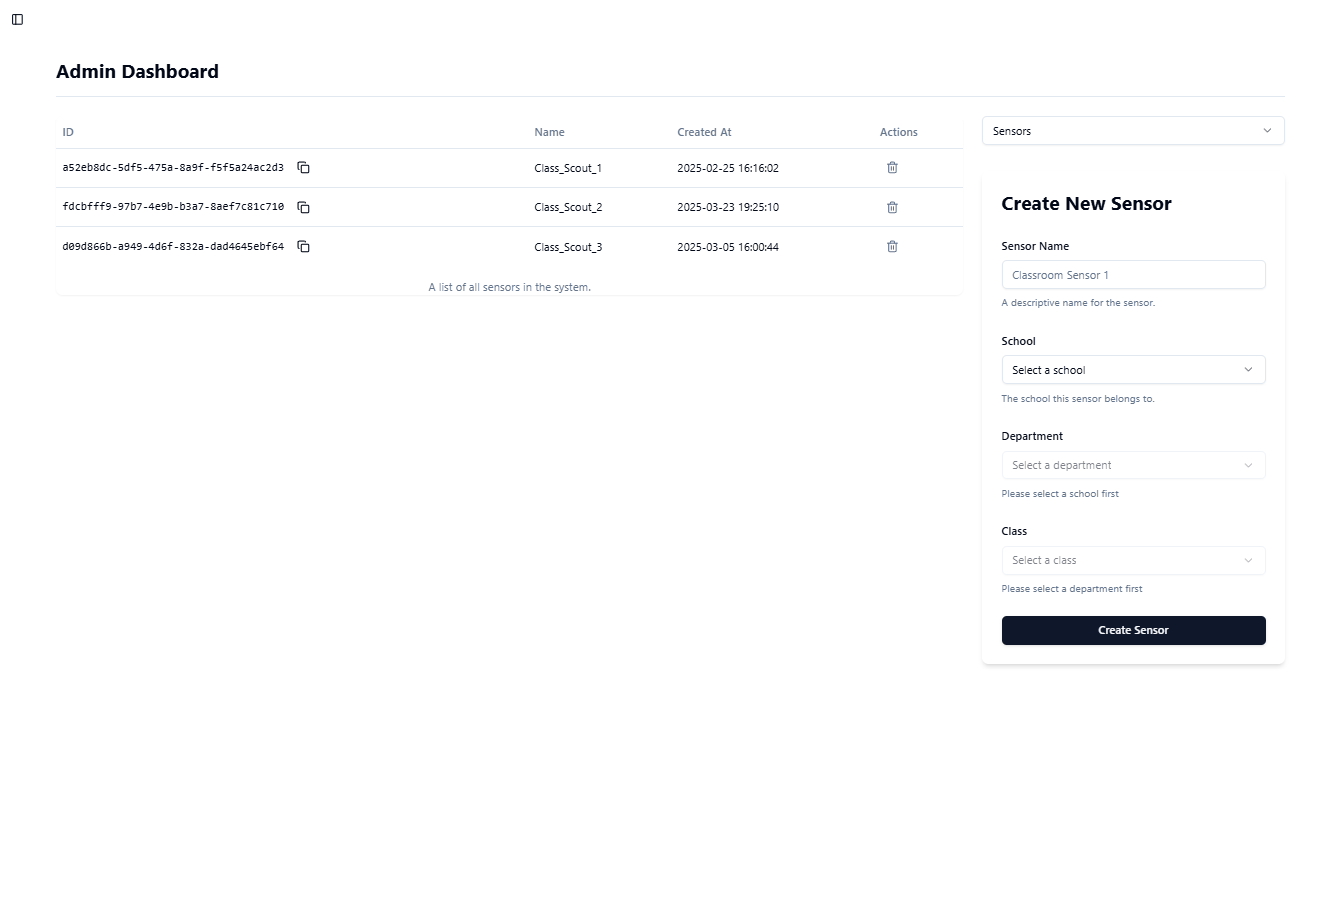
\includegraphics[width=1\textwidth]{files/Thomas/pics/Website/admin/devices/devices-screen.png}
\caption[Bildbezeichnung für Abbildungsverzeichnis]{}
\label{fig:gehaeuse_internet_bild}
\end{figure}

\clearpage


In dem Bild kann man sehen wie das Dashboard der Sensoren ausschaut.

\subsection{Tabele}

Jeder Table hat außer die User Table die ist speziel hat am anfag die uuid von den Strukturelementen. Diese Last sich immer ganz einfach kopiern durch einen Button. Danach wird der Name angezeigt und nachdem wird der Zeitpunkt der Erstellung des Strukturelementes angeziegt und am schluss eine Möglichkeit diese Strukturelemente zu löschen. 


%%% code hinzufügen 

\subsubsection{School Table}

google



\subsection{Erstellen}

Beim Erstellen muss sich 





\newpage

\section{Backend}





\begin{figure}[!htb]
\centering
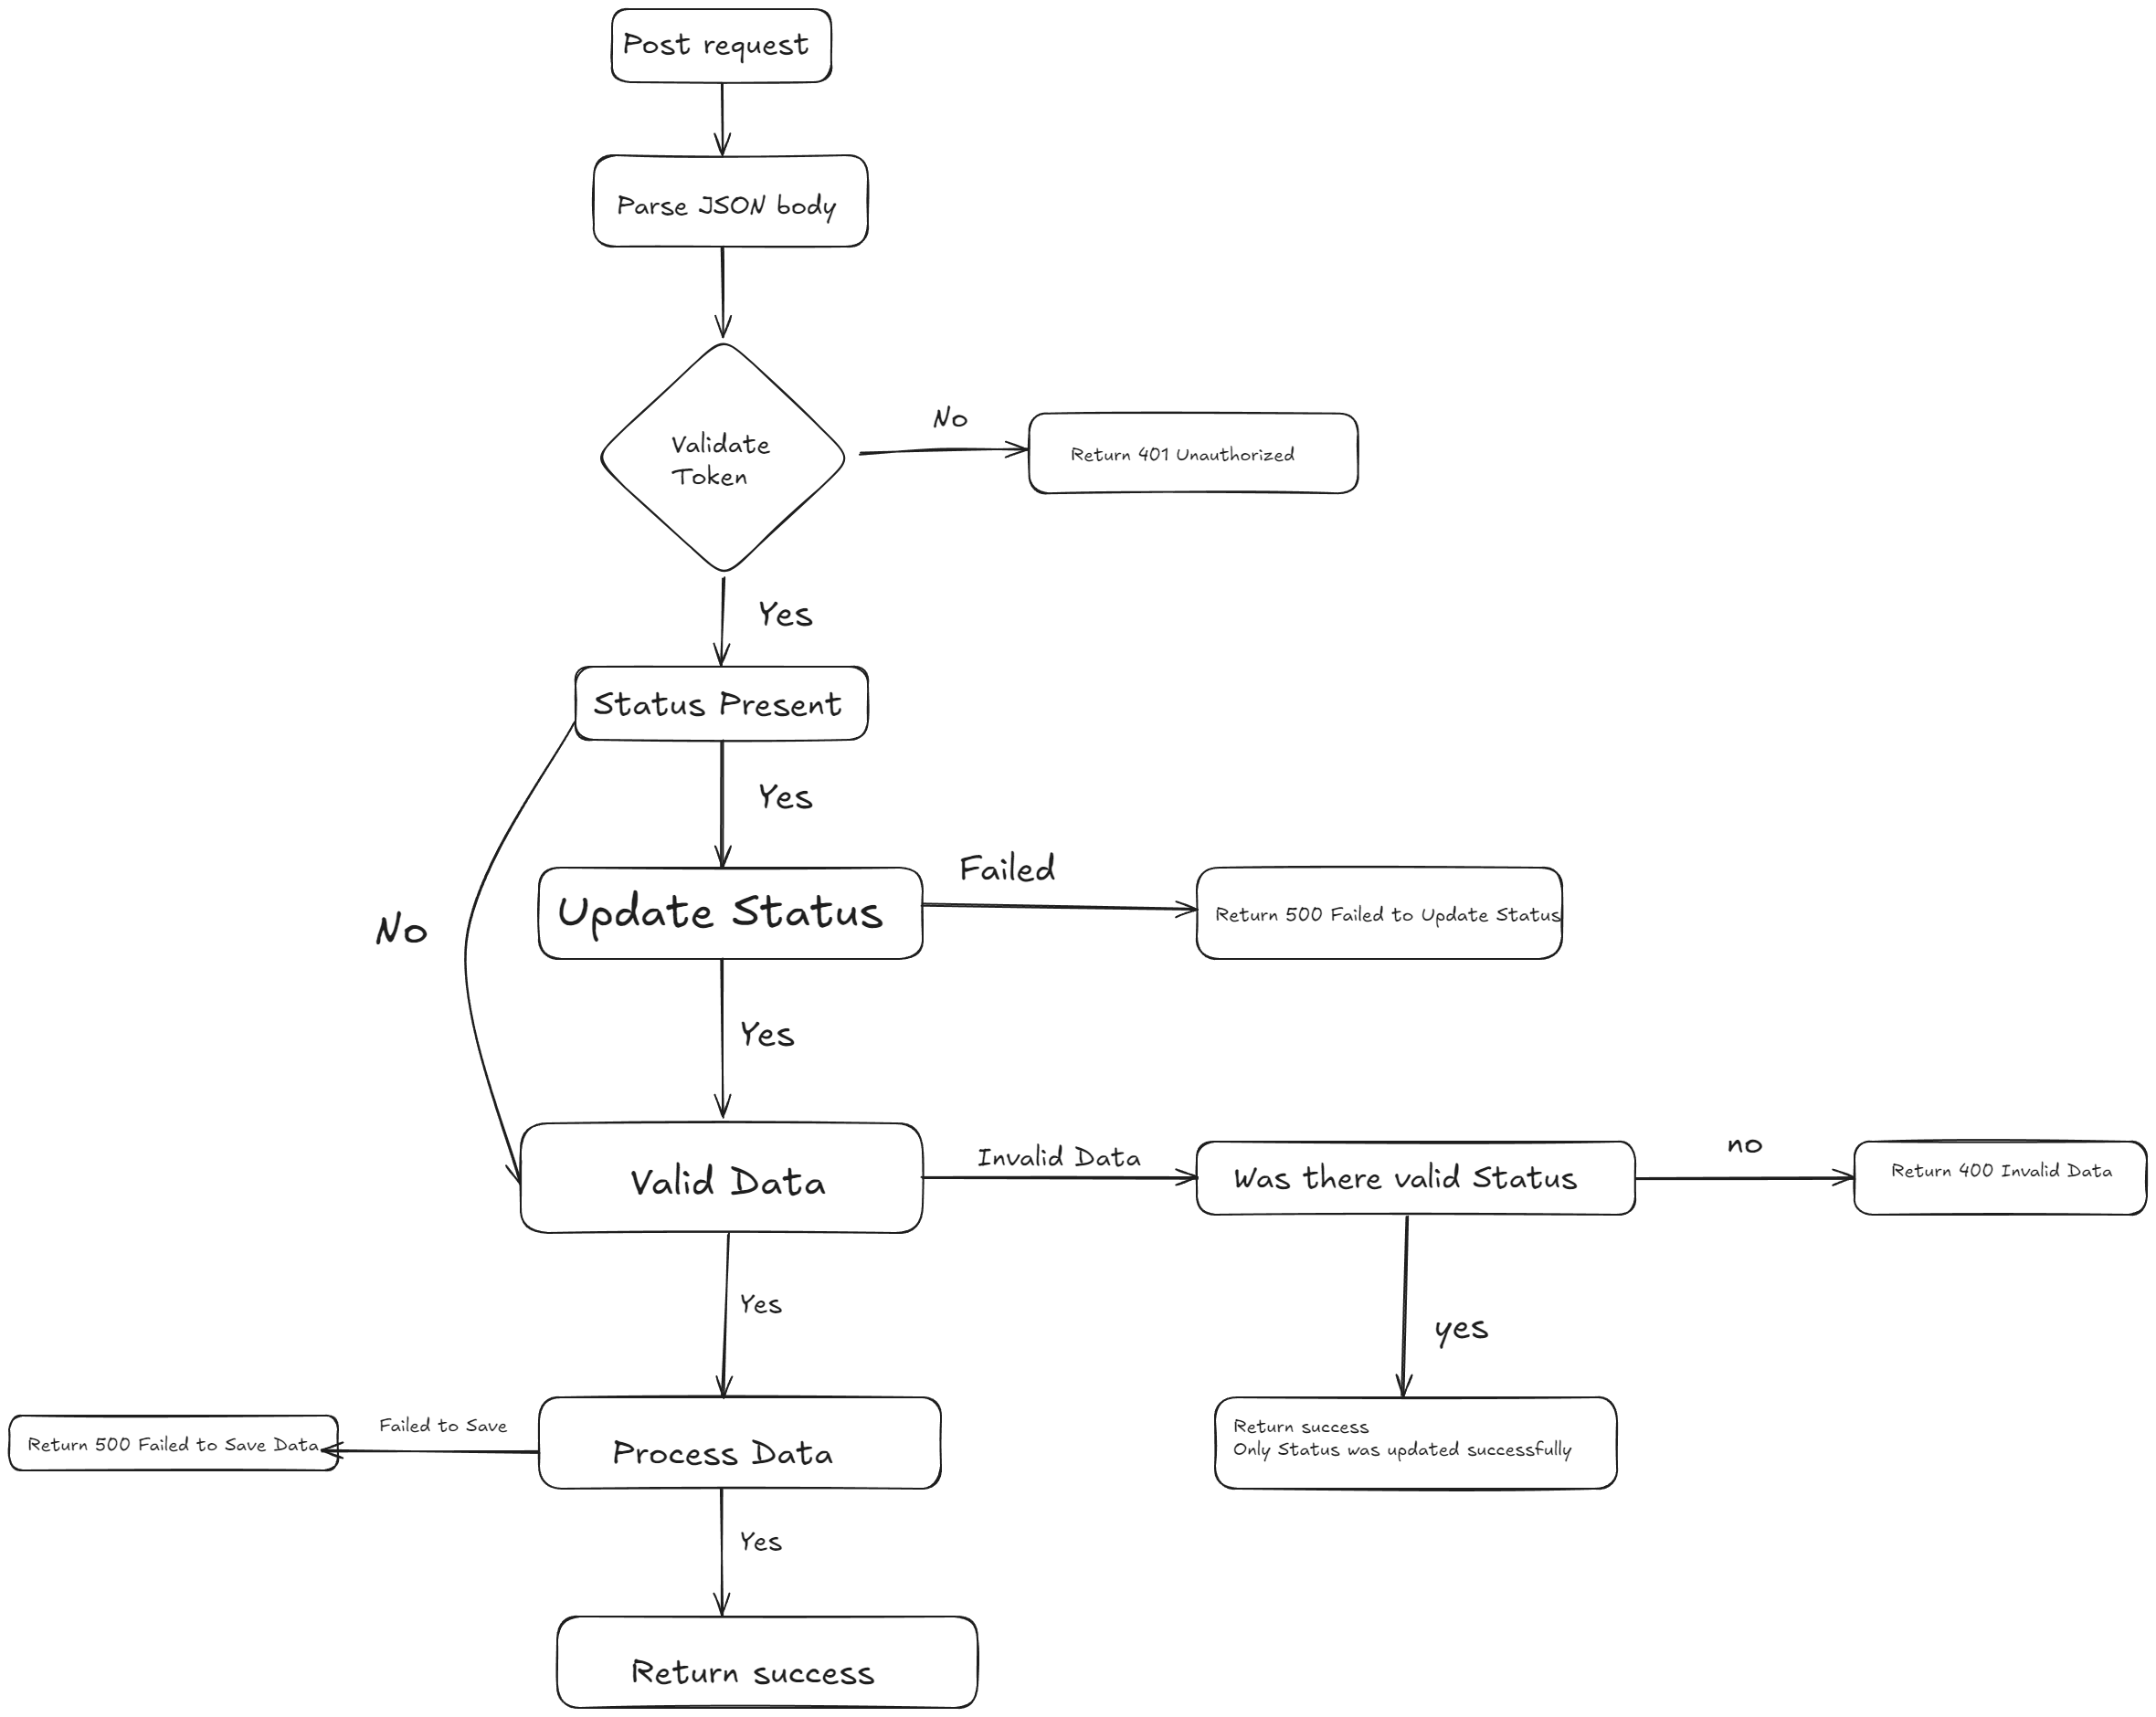
\includegraphics[width=1\textwidth]{files/Thomas/pics/Website/backend/image.png}
\caption[Bildbezeichnung für Abbildungsverzeichnis]{}
\label{fig:gehaeuse_internet_bild}
\end{figure}

\clearpage





\end{inhalt}